\chapter{Related Work \label{related_work_chapter}}
In this chapter, we present a brief review of the literature related to the concepts that we discuss in this thesis.

\section{Volume Rendering \label{volume_rendering}}
%Volume rendering is used to display a 2D image of a three-dimensional (3D) data set. It can be considered as a projection of a 3D volumetric data set into a two-dimensional (2D) image \cite{garcia_parallel_2006}.
%% without extracting intermediate polygonal representations \cite{garcia_parallel_2006}.
%The majority of data sets are discretely sampled along 3D grids and contain scalar values usually acquired from medical imaging devices such as CT or MRI machines or various scientific simulations such as fluid simulation.
%The data then takes the form a 3D array of voxels (a three dimensional extension of pixels).
%%There are various kinds of volumetric data sets. Typical volumetric data sets in medical visualization are groups of two-dimensional (2D) slice images acquired by a CT, MRI, or MicroCT scanner.
%In flow visualization, the data sets are often generated from simulations.
%Volume rendering is called direct volume rendering, where no polygonal representations are generated in the process, whereas rendering from polygonal representations extracted from volumetric data sets is called indirect volume rendering.
%Volume rendering can be performed using two main techniques, either by extracting a number of surfaces from the data and rendering these surfaces to the screen, called isosurface rendering or by rendering the volume itself as a complete block of data with no intermediary structures, usually called direct volume rendering (DVR).

Volume rendering is used to display a two-dimensional (2D) image of three-dimensional (3D) data set. It can be considered as a projection of a 3D volumetric data set to a 2D image \cite{garcia_parallel_2006}.
The majority of data sets are discretely sampled along 3D grids and contain scalar values usually acquired from medical imaging devices such as CT or MRI machines or computed from scientific simulations such as fluid simulation.
The data sets have the form of 3D arrays and the elements in the data sets are called voxels, which correspond to pixels in 2D images.
An example of volume rendering is provided in Figure~\ref{fig:multiple_VisMale}, which shows a sliced image and a volume rendered image of a head data set.

%\begin{figure}
%	\centering
%	\begin{minipage}{0.25\textwidth}
%		\centering
%		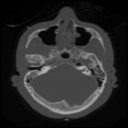
\includegraphics[width=1\linewidth]{images/VisMale_slice.jpg}
%		\caption{A sliced image of the data set}
%		\label{fig:VisMale_slice}
%	\end{minipage}~
%	\begin{minipage}{0.25\textwidth}
%		\centering
%		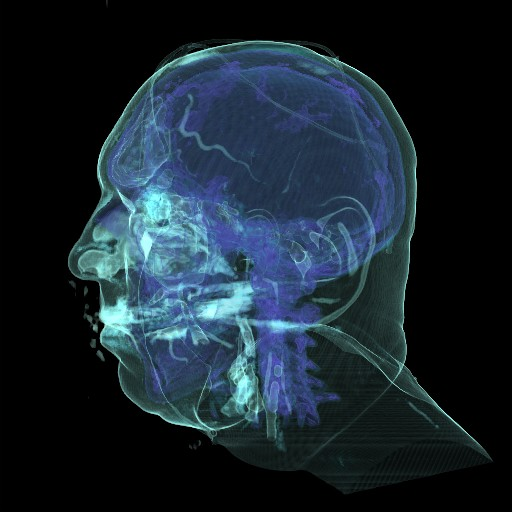
\includegraphics[width=1\linewidth]{images/VisMale.jpg}
%		\caption{Volume rendering of the data set}
%		\label{fig:VisMale}
%	\end{minipage}
%	\caption{The VisMale data set \cite{website:Roettger_volume_2013}}
%	\label{fig:multiple_VisMale}
%\end{figure}

Traditionally, volume rendering techniques are categorized as direct volume rendering and indirect volume rendering.
Indirect volume rendering is done be extracting surfaces from the data sets and rendering these surfaces, while direct volume rendering render the volume data set as a complete block of data without extracting intermediary structures.
Since indirect volume rendering is not in the scope of this thesis, direct volume rendering would henceforth be referred to as volume rendering.

Volume visualization is another term for volume rendering, sometimes with emphasis on the realistic aspects of volume rendering. In addition to the realistic aspects of volume rendering, there is non-photorealistic volume rendering, which emphasizes the illustrative and artistic aspects of volume rendering.
Volume visualization was initially used in medical imaging, and later became an essential techinque in many sciences for portraying complex phenomena such as clouds, water flows, and molecular and biological structure \cite{rosenblum_scientific_1994}.

\begin{figure}
\centering
\begin{minipage}{.25\textwidth}
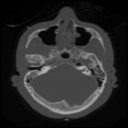
\includegraphics[width=1\linewidth]{images/VisMale_slice.jpg}
\caption{A sliced image of the data set}
\label{fig:VisMale_slice}
\end{minipage}~
\begin{minipage}{.25\textwidth}
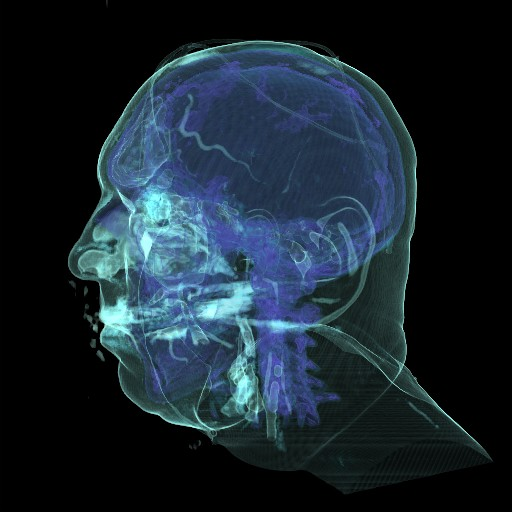
\includegraphics[width=1\linewidth]{images/VisMale.jpg}
\caption{Volume rendering of the data set}
\label{fig:VisMale}
\end{minipage}
\caption{The VisMale data set \cite{website:Roettger_volume_2013}}
\label{fig:multiple_VisMale}
\end{figure}

%Whereas rendering from polygonal representations extracted from volumetric data sets is also called indirect volume rendering.

%There are four typical volume rendering techniques: ray casting, splatting, shear warp and texture mapping. In recent years, many variants and combinations of these techniques have been proposed, especially approaches which utilise GPU hardware to improve performance or even achieve real-time interactivity.

%A volume renderer maps every voxel (an element in volume data) to an opacity and a color with a transfer function, which is a piecewise linear function or an arbitrary table. Once converted to an RGBA value, the composed RGBA result is projected on corresponding pixel of the frame buffer with certain volume rendering techniques.

\subsubsection{Non-Photorealistic Rendering (NPR)}
In contrast to traditional computer graphics, which has focused largely on creating photorealistic images of synthetic objects, non-photorealistic rendering (NPR) is an area of computer graphics that focuses on creating abstract images with a wide variety of expressive styles \cite{haeberli_paint_1990}. NPR has been an active research area for a long time. A number of approaches have been proposed to produce convincing artistic styles for both off-line and on-line rendering. For example, there are various types of commonly used styles including painterly rendering, edge stylization, sketch-shading, cel-shading, hatching.
% Although there are plenty of works on non-photorealistic rendering, most of them focus on how to imitate artistic styles with emphasis on aesthetic aspects.
%Researchers in modelling and rendering in computer graphics have focused for many years on producing photorealistic images, which are indistinguishable from photographs captured from real-world scene. Nevertheless, there are other compelling methods of visual discourse such as paintings, sketches and cel animation.
In certain situations, non-photorealistic renderings are considered more effective and expressive than an equivalent photograph \cite{healey_perceptually_2004}.

%As a basic part of most approaches to non-photorealistic volume rendering, contours delineate object shape and clarify sites of occlusion by emphasizing the transition between front-face and back-facing surface locations.
%Kindlmann et al. \cite{kindlmann_curvature-based_2003} proposed curvature-based transfer function to enhance the expressive and informative power of volume rendering. In their approach, volume data is rendered with contours to exhibit constant thickness in image space.

\subsubsection{Illustrative Volume Visualization}
NPR models were adopted in visualization and hence formed the field illustrative visualization.
Illustrative visualization, as a novel category of visualization, aims at visualizing data in a clear and understandable way using techniques from traditional hand-crafted illustrations.
Illustrative visualization has been successful employed in medical visualization \cite{svakhine_illustration_2005} \cite{viola_importance-driven_2005} \cite{svakhine_illustration-inspired_2009}.

Illustration-based styles are believed to be effective in conveying information. Researchers in the field of computer graphics and visualization have applied illustration-based styles in order to produce effective and expressive visualization. Stompel et al. \cite{stompel_visualization_2002} introduced feature enhancement techniques, such as strokes based, temporal domain enhancement, to enhance time-varying data obtained from the field of computational fluid dynamics (CFD).

In scientific visualization, features of interest are often inner structures of the data sets, e.g. visualizing certain structures in anatomical data sets \cite{diaz_iriberri_enhanced_2013}.
Inspired by techniques from illustration, various approaches are proposed to reveal different level of structures simultaneously in volume data sets.
Two level rendering \cite{hauser_two-level_2001} \cite{hadwiger_high-quality_2003} \cite{corcoran_perceptual_2010} is a method of merging several volume rendering techniques into a single rendering. This method is useful when inner structures needs to be rendered along with semitransparent outer parts.
Focus and context \cite{wang_magic_2005} \cite{bruckner_illustrative_2006} \cite{chen_intelligent_2008} provides a means of revealing the interior of a volume data set in a feature-driven way and also retaining context information.
Another alternative is the cutaway technique \cite{burns_feature_2007} \cite{sigg_intelligent_2012}, which makes inner structures clearly visible along with its spatial relation to the surrounding material.

\subsubsection{Other NPR Techniques in Volume Visuailzation \label{painterly_rendering}}
Streamlines and textures are often used to represent flow directions \cite{urnessy_techniques_2004}. Interrante and Grosch \cite{interrante_strategies_1997} introduced volume LIC (Line Integral Convolution) to visualize 3D flow via volume textures.
%Figure~\ref{fig:interrante_strategies_1997} shows a volume texture generated with LIC. In this figure, vorticity magnitude is mapped to streamline color and the striations along the axial direction reveal the presence of periodic waves propagated down the jet axis.
Since volume LIC is limited to steady flows, Liu and Moorhead \cite{liu_texture-based_2005} introduced an accelerated unsteady flow LIC algorithm to generate volume flow textures.
% (Figure~\ref{fig:liu_texture-based_2005}).
In their approach, magnitude-based transfer functions and cutting planes in volume rendering are employed to show the flow structure and the flow evolution.

Artists recognize patterns and flows in a target scene and express them through brush strokes. They use stroke orientation corresponding to the actual movement \cite{lee_motion_2009}. This type of techniques from master painting and human perception are used to visualize multidimensional data sets \cite{healey_perceptually_2004}. Tateosian et al. \cite{tateosian_engaging_2007} use the color, orientation and size of strokes to represent the magnitude, flow orientation and pressure of a 2D slice of a simulated supernova collapse.
% (Figure~\ref{fig:tateosian_engaging_2007}).
Lee et at. \cite{lee_motion_2009} presented a painterly rendering technique based on the motion information (magnitude, direction, standard deviation) extracted from an image sequences of the same view.
Besides stroke-based techniques and texture-based techniques, particle-based techniques \cite{busking_particle-based_2007} \cite{van_pelt_illustrative_2010} were also proposed to produce user-configurable stylized renderings from volume data sets, imitating traditional pen and ink drawings.

%\begin{figure}
%	\centering
%	\begin{minipage}{.49\textwidth}
%		\centering
%		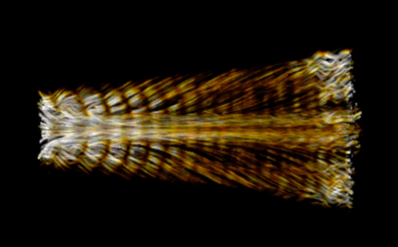
\includegraphics[width=1\linewidth]{images/interrante_strategies_1997.png}
%		\caption{Streamlines are represented as a volume texture, which provides an intuitive impression of the 3D flow. \cite{interrante_strategies_1997}}
%		\label{fig:interrante_strategies_1997}
%	\end{minipage}~
%	\begin{minipage}{.49\textwidth}
%		\centering
%		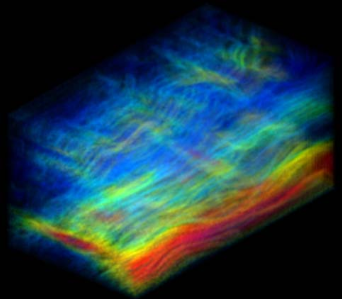
\includegraphics[width=1\linewidth]{images/liu_texture-based_2005.png}
%		\caption{Streamlines are represented as a volume texture, which provides an intuitive impression of the 3D flow. \cite{liu_texture-based_2005}}
%		\label{fig:liu_texture-based_2005}
%	\end{minipage}
%\end{figure}
%
%\begin{figure}
%	\centering
%	\begin{minipage}{.49\textwidth}
%		\centering
%		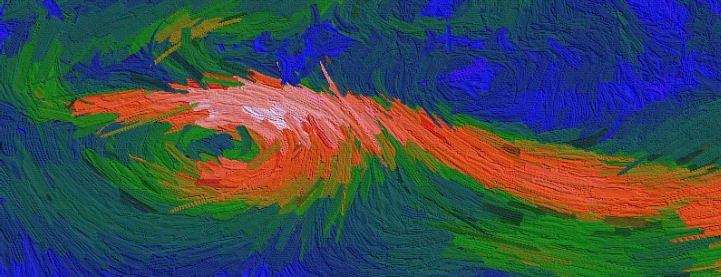
\includegraphics[width=1\linewidth]{images/tateosian_engaging_2007.png}
%		\caption{A visual complexity style visualization of flow patterns in a 2D slice though a simulated supernova collapse, using the mappings: flow orientation $ \rightarrow $ stroke orientation, magnitude $ \rightarrow $ order and pressure $ \rightarrow $ stroke size \cite{tateosian_engaging_2007}.}
%		\label{fig:tateosian_engaging_2007}
%	\end{minipage}~
%	\begin{minipage}{.49\textwidth}
%		\centering
%		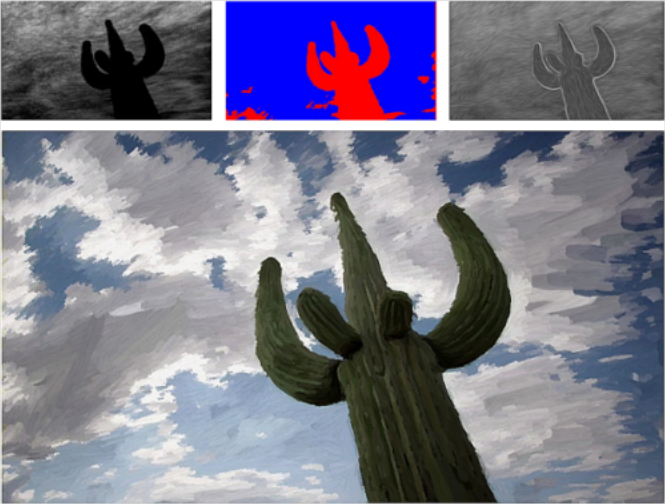
\includegraphics[width=1\linewidth]{images/lee_motion_2009.png}
%		\caption{The motion directions determine stroke orientations in the regions with significant motions, and image gradients determine stroke orientations where little motion is observed \cite{lee_motion_2009}.}
%		\label{fig:lee_motion_2009}
%	\end{minipage}
%\end{figure}

\section{Transfer Functions \label{literature_of_transfer_function}}
Volume data are 3D entities with information inside them, but the data might not consist of surfaces and edges.
%, or might be too voluminous to be represented geometrically.
%The goal of volume visualization is to gain insightful depictions of volume data.
Because of the lack of explicit geometric information, %and limited semantics, 
it is a major challenge to provide clear visualizations of the structures contained in a volume dataset.
Volume data may be rendered directly by mapping scalar values to visual properties (e.g. opacity and color), or an intermediate geometric representation may be extracted using techniques like Marching Cubes \cite{lorensen_marching_1987} and then rendered as geometric surfaces. The mapping, which assigns visual properties to volume data, is called a transfer function.

Transfer function specification is an essential part in volume visualization.
%In terms of dimensionality, transfer functions are divided into two categories, one-dimensional (1D) and multidimensional.
A simple one-dimensional transfer function is a mapping from scalar values to RGB and alpha values.
The resulting visualization largely depends on how well the transfer function captures features of interest \cite{kniss_multidimensional_2002}.
%Due to the complex nature of volumetric data sets, abstraction techniques is often used in order to provide better understanding of the data sets.
However, it is non-trivial to obtain an effective transfer function. The specification is often a trial-and-error process, which involves a significant amount of tweaking of color and opacity. Figure~\ref{fig:multiple_glk_transfunction} shows how slight changes in the transfer function lead to significant changes in the resulting images. The adjustment of transfer functions is unintuitive and often difficult.

\begin{figure}
        \centering
        \begin{minipage}{0.5\textwidth}
                \centering
                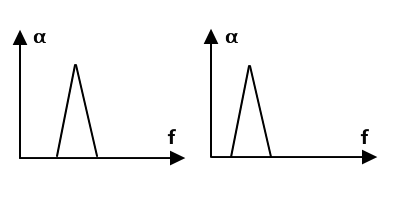
\includegraphics[width=1\linewidth]{images/glk_transfunction_tf.png}
                \caption{Two transfer functions (TF)}
                \label{fig:glk_transfunction_tf}
        \end{minipage}~
        \begin{minipage}{0.25\textwidth}
                \centering
                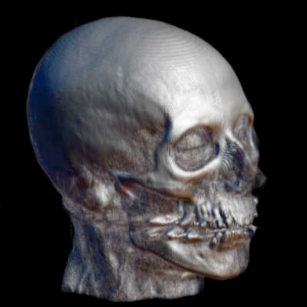
\includegraphics[width=1\linewidth]{images/glk_transfunction_1.png}
                \caption{The result from the TF on the left in \ref{fig:glk_transfunction_tf}}
                \label{fig:glk_transfunction_1}
        \end{minipage}~
        ~ %add desired spacing between images, e. g. ~, \quad, \qquad etc.
          %(or a blank line to force the subfigure onto a new line)        
        \begin{minipage}{0.25\textwidth}
                \centering
                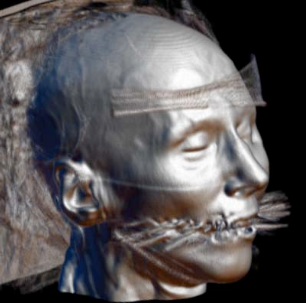
\includegraphics[width=1\linewidth]{images/glk_transfunction_2.png}
                \caption{The result from the TF on the right in \ref{fig:glk_transfunction_tf}}
                \label{fig:glk_transfunction_2}
        \end{minipage}    
        \caption{Slight changes in the transfer function causes significant difference in the resulting images \cite{kindlmann_transfer_2002}}
        \label{fig:multiple_glk_transfunction}
\end{figure}

In practice, major factors that have a great influence on transfer function setting are: partial volume effect \footnote{During the acquisition of data, the finite resolution causes contributions of different materials combined into the value of a single voxel. This is generally referred to as the partial volume effect, which results in blurred boundaries and hampers the detection of small or thin structures. \cite{serlie_classifying_2007}}, non-uniform distribution of materials and noise \cite{serlie_computed_2003}.
Among these, two challenging problems that need to be tackled could be elaborated as follows: firstly, for volume data sets, e.g. those obtained by MRI and CT, different tissues are represented in similar or even overlapping ranges of scalar values; secondly, interesting interior structures are often partly or completely occluded by surrounding tissue.
%This is common in visualizing interior structures. 
Consequently, feature detection and understanding volume data become a big challenge.

These problems are handled by transfer functions, which have played a crucial role in volume visualization.
%Transfer functions have played a crucial role in volume visualization.
Good transfer functions reveal important structures in the data without obscuring them with less important regions.
%Traditional one-dimensional transfer function approaches, which assign optical properties only based on scalar value, are inadequate to extract inner structures of interest from volume data.
%Various strategies have been proposed to simplify transfer function specification \cite{pfister_transfer_2001}.
The design of transfer functions to generate informative visualizations has been a significant challenge addressed by a number of researchers \cite{pfister_transfer_2001}.
Various strategies have been proposed for transfer function design \cite{hadwiger_real-time_2006}.
%Data-centric strategies examine the properties of volume data sets.
Data-centric strategies examine the properties of volume data sets.
However, certain features are difficult to be extracted and visualized with 1D transfer functions, e.g. CT and MRI data sets which contain complex boundaries between multiple materials.
Overlapping intensity intervals corresponding to different materials make boundary separation difficult.
When one intensity value or interval is associated with multiple boundaries, a 1D transfer function is unable to render them in isolation \cite{kniss_multidimensional_2002}.
%Overlapping intensity intervals corresponding to different materials make boundary detection difficult.
%However, certain features of interest in volume data are difficult to extract and visualize with 1D transfer functions. For instance, many medical data sets created from CT or MRI scans contain a complex combination of boundaries between multiple materials. This situation is problematic for 1D transfer functions because of the potential for overlap between the data value intervals spanned by the different boundaries. When one data value or data range is associated with multiple boundaries, a 1D transfer function is unable to render them in isolation \cite{kniss_multidimensional_2002}.

Classical approaches to this problem try to detect boundary information between tissues by introducing derived attributes such as first and second-order derivatives to isolate materials \cite{kindlmann_semi-automatic_1998} \cite{kniss_multidimensional_2002}. In this case, the transfer functions are extended to multidimensional feature spaces. 
The introduction of multidimensional transfer functions alleviates the material separation problem.
Instead of classifying a sample based on a single scalar value, multi-dimensional transfer functions allow a sample to be classified based on a combination of values.
Multidimensional transfer functions are very effective means to extract materials and their boundaries for both scalar and multivariate data. However, the parameter spaces of multidimensional transfer functions are more complex (compared to 1D transfer functions) and thus introduce problems such as requirement for large amount of user interaction, missing precision or the interaction being complex and unintuitive \cite{arens_survey_2010}.
%As a result, the interaction of transfer functions becomes more complex and unintuitive.

There are other multi-dimensional transfer functions approaches, such as spatialized gradient-based transfer functions \cite{roettger_spatialized_2005}, distance-based transfer functions \cite{tappenbeck_distance-based_2006}, size-based transfer function \cite{correa_size-based_2008}, texture-based transfer functions \cite{caban_texture-based_2008} \cite{alper_selver_exploring_2015} and curvature based transfer functions \cite{kindlmann_curvature-based_2003}.
Bruckner and Gr{\"o}ller introduced the concept of style transfer functions \cite{bruckner_style_2007}, which aim to produce more comprehensible images by using transfer functions that map input values to different NPR rendering styles.

Another strategy is based on the selection of rendered images. This strategy lets the user select one or more favorite images to guide the further search of transfer functions \cite{marks_design_1997} \cite{wu_interactive_2007}. More recent approaches introduced visibility \cite{correa_visibility_2011} or measures derived from information theory \cite{haidacher_information-based_2008} \cite{bruckner_isosurface_2010} \cite{ruiz_automatic_2011} \cite{bramon_information_2013}. Zhou et al. \cite{zhou_transfer_2012} studied the combination of 2D transfer functions with occlusion and size-based transfer functions.

Despite the advances of these methods, transfer function design for volume rendering is still an open research problem.
The creation of transfer functions needs to be simplified and the functionality of transfer functions needs to be extended in order to realize the full potential of volume rendering. For instance, more sophisticated transfer functions are required in medical imaging, in order to address various domain specific visualization problems \cite{lindholm_spatial_2010}.

Moreover, transfer function specification in general is an unintuitive or even monotonous task for average users, because it is usually an iterative process of trial and error.
For instance, there are skin and fat tissues around the brain, and their intensities lie in the same range as the brain. If we want to visualize the brain by setting the scalar value range of the brain to opaque, the surrounding skin and fat tissue will also become opaque. Then the brain will be occluded by the surrounding soft tissues which make it difficult to explore the brain structure.
Common approaches to this problem are to introduce explicit segmentation of structures of interest before the volume rendering process \cite{rezk-salama_opacity_2006}. In fact, the process of applying the transfer function could be interpreted as a segmentation problem.

\subsection{Multidimensional Transfer Functions}
Multidimensional transfer functions \cite{kniss_interactive_2001}, which are mappings from intensity and other variables, such as first and second derivatives to color and opacity, have demonstrated their effectiveness in distinguishing boundaries between materials in volume data.

%Overlapping intensity intervals corresponding to different materials make boundary detection difficult. Classical approaches try to detect boundary information between tissues by introducing derived attributes such as first and second derivatives to isolate materials \cite{kindlmann_semi-automatic_1998} \cite{kniss_multidimensional_2002} \cite{kindlmann_transfer_2002}.
%In this case, the transfer functions are extended to multidimensional feature spaces. As a result, the interaction of transfer functions becomes more complex and unintuitive as the dimensionality becomes higher.
%%Even two-dimensional transfer functions require a considerable amount of user interaction to find a meaningful shape \cite{arens_survey_2010}.

In volume data, boundaries are regions between areas of relatively homogeneous material. It is difficult to detect boundaries because different materials often consist of overlapping intensity intervals. To address this problem, multidimensional transfer functions used derived attributes such as gradient magnitudes and second derivatives along with scalar values, in order to detect transitions between relatively homogeneous areas \cite{kindlmann_semi-automatic_1998} \cite{kniss_multidimensional_2002} \cite{kindlmann_transfer_2002}.
%Classical approaches try to detect boundary information between tissues by introducing derived attributes such as first and second derivatives to isolate materials \cite{kindlmann_semi-automatic_1998} \cite{kniss_multidimensional_2002} \cite{kindlmann_transfer_2002}.
In this case, the transfer functions are extended to multidimensional feature spaces.
For higher-dimensional transfer functions, the generation of transfer functions could be memory intensive and costly to compute,
%and exploration of the transfer function domain might not be intuitive.
and the interaction of transfer functions becomes more complex and unintuitive as the dimensionality becomes higher. 
%As a result, the interaction of transfer functions becomes more complex and unintuitive as the dimensionality becomes higher.

Therefore, two-dimensional (2D) histograms are often used in multidimensional transfer functions \cite{maciejewski_structuring_2009}. An example is a 2D histogram with axes representing a subset of the feature space (e.g. scalar value vs gradient magnitude), with each entry in the 2D histogram being the number of voxels for a given feature space pair.
%A great number of transfer function approaches have also been merged and one-dimensional transfer function is extended to multi-dimensional transfer function.
Even in the case of two-dimensional transfer functions, a considerable amount of user interaction is required in order to come up with meaningful results \cite{arens_survey_2010}.
%Even in the case of two-dimensional transfer functions, a considerable amount of user interaction is required in order to come up with meaningful results \cite{arens_survey_2010}.
%There are other multi-dimensional transfer functions approaches, such as spatialized gradient-based transfer functions \cite{roettger_spatialized_2005}, distance-based transfer functions \cite{tappenbeck_distance-based_2006}, size-based transfer function \cite{correa_size-based_2008}, texture-based transfer functions \cite{caban_texture-based_2008} and curvature based transfer functions \cite{kindlmann_curvature-based_2003}.

As one of the most common representations of voxel distributions, histograms are used in transfer function design to assign visual properties to voxels \cite{pfister_transfer_2001}. Bajaj et al. \cite{bajaj_contour_1997} introduced the contour spectrum to determine voxels corresponding to important isosurfaces in the volume. To overcome the difficulty of using one-dimensional transfer functions (solely based on scalar values stored in the voxels) to extract inner structures of interest from the volume data, Levoy proposed the use of gradient magnitude to emphasize strong boundaries between different tissues \cite{levoy_display_1988}.

The introduction of gradient magnitude as a data metric aims to detect voxels that are of large deviation compared with other voxels by approximating gradient magnitude at each sample point in the volume, because the exact distribution of data is unknown due to information lost in the discrete sampling process.

Kindlmann and Durkin extended Levoy's work by introducing a higher dimensional transfer function domain based on gradient magnitudes and second derivatives \cite{kindlmann_semi-automatic_1998}. To emphasize different structures, Kniss et al. \cite{kniss_interactive_2001} presented a technique for interactively manipulating 2D histograms of gradient magnitudes and data values. In their work, material boundaries appear as arcs in the 2D histogram and can be selected with interactive widgets \cite{kniss_multidimensional_2002}.
Kindlmann et al. \cite{kindlmann_curvature-based_2003} proposed curvature-based transfer function to enhance the expressive and informative power of volume rendering. In their approach, volume data is rendered with contours to exhibit constant thickness in image space.
Maciejewski et al. proposed a non-parametric method to generate transfer function \cite{maciejewski_structuring_2009}.
In their later work \cite{maciejewski_abstracting_2013}, instead of using the attributes, metrics representing relationships and correlations in the underlying data were used in the method.
Wang et al. introduced clustering of 2D density plots in their automating transfer function \cite{wang_automating_2012}.
Ip et al. \cite{ip_hierarchical_2012} described a multilevel segmentation technique that mimics user exploration behaviors by recursively segmenting intensity-gradient histograms. The use of parallel coordinates is introduced to assist the design of transfer functions in multidimensional parameter spaces \cite{zhao_multi-dimensional_2010} \cite{guo_multi-dimensional_2011}.

\subsection{Transfer Functions for Time-Varying Volume Visualization}
Although researchers have developed a great number of visualization techniques for time-invariant volume data, how to effectively explore and understand time-varying volume data remains a challenging problem. Finding good transfer functions for time-invariant volume data itself has proven difficult \cite{pfister_transfer_2001}.
%Finding good transfer functions for time-varying volume data is even more difficult, as data value ranges and distributions change over time.
%Although researchers have developed a great number of visualization techniques for static volume data, how to effectively explore and understand time-varying volume data remains a challenging problem.
Finding good transfer functions for time-varying volume data is more difficult than for static volume data, as data value ranges and distributions change over time.

Coherence is an important issue of transfer function design for time-varying volume data. Ideally, a single transfer function should be used for the whole time-varying data set in order to obtain coherent visualization. More than one color or opacity map can be misleading or physically meaningless, because the transition from one transfer function to another may cause sudden changes in the resulting images. However, this practice is not always applicable to general time-varying data sets.

Volume data sets are inherently 3D representations. Automated analysis methods, such as temporal trends or statistical aggregates e.g. mean values and standard deviations, are often applied in order to abstract dynamic characteristics of the data sets \cite{kehrer_visualization_2013}.

%Jankun-Kelly and Ma \cite{jankun-kelly_study_2001} examined how to combine transfer functions for different time-steps to generate a coherent transfer function.
Jankun-Kelly and Ma \cite{jankun-kelly_study_2001} examined how to combine transfer functions for different time-steps to generate a coherent transfer function.
Woodring et al. \cite{woodring_high_2003} considered time-varying volume data as four-dimensional data field and provided a user interface to specify hyperplanes in 4D.
Woodring and Shen \cite{woodring_chronovolumes_2003} introduced an alternative approach to render multiple time-steps in a sequence with different colors into a single image. This approach provides the context of surrounding time steps but coherence of color among time-steps is hard to maintain.
%Tikhonova et al. \cite{tikhonova_exploratory_2010} presented an exploratory approach based on a compact representation of each time step of the dataset in the form of ray attenuation functions. Ray attenuation functions are subsequently used for transfer function generation.
Tikhonova et al. \cite{tikhonova_exploratory_2010} presented an exploratory approach based on a compact representation of each time step of the dataset in the form of ray attenuation functions. Ray attenuation functions are subsequently used for transfer function generation.
Akiba et al. \cite{akiba_simultaneous_2006} introduced the time histogram which allows simultaneous classification and specification of temporal transfer functions for the entire time series.

A time-varying volume data set can be considered as a 3D array where each voxel contains a time-activity curve (TAC). Fang et al. \cite{fang_visualization_2007} described an approach for classifying time-varying volume data based on the temporal behavior of voxels and three different similarity measures that can be used in their approach.
Woording and Shen \cite{woodring_multiscale_2009} presented a method that filters time-varying volume data into several time scales using wavelet transform and classifies the voxels by clustering the entire time series by time scale.
Lee and Shen \cite{lee_visualizing_2009} proposed a method for classifying time-varying features using time activity curves with the dynamic time warping distance metric.
Woodring et al. \cite{woodring_semi-automatic_2009} utilized a method called temporal clustering and sequencing to find dynamic features in value space and create dynamic transfer functions through time-series analysis.
Ward and Guo \cite{ward_visual_2011} presented a method for visualizing time-series data that reveals a wide variety of features in the data, by mapping short sub-sequences of the time-varying volume data into a high-dimensional shape space, and then performing a dimension reduction process to allow projection into screen space.
Gu and Wang \cite{gu_transgraph:_2011} proposed an approach to organize a time-varying data set into a hierarchical graph, which captures the transition relationships in the data set. This approach assists the user in comprehending the correspondence between volume regions over time and allows interaction of the graph through brushing and liking.

\begin{figure}
\centering
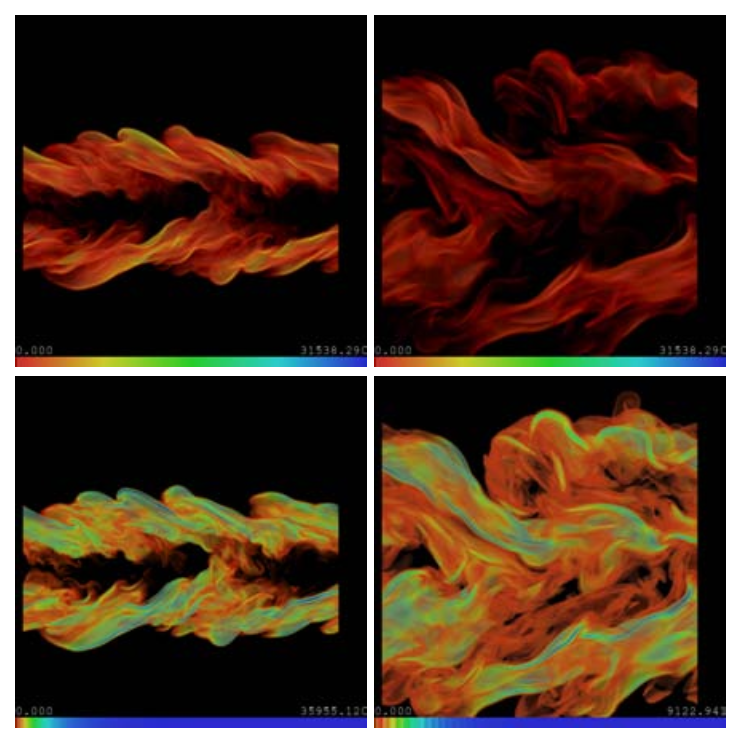
\includegraphics[width=1\linewidth]{images/woodring_semi-automatic_2009}
\caption{A single static transfer function cannot capture dynamic features. In the two images at the top, the features appear to vanish over time. On the other hand, the features are visible over time if a dynamic transfer function is used (the two images at the bottom) \cite{woodring_semi-automatic_2009}.}
\label{fig:woodring_semi-automatic_2009}
\end{figure}

\subsubsection{Visualising Time-Varying Volume Data with NPR}
An essential problem in time-varying volume visualization is to visualize temporal variation and analysis of features. Traditionally, time-varying data has been visualized as snapshots of individual time steps or animation of snapshots of a sequence of time steps. These techniques are effective in making time-varying data understandable. However, they struggle when the complexity of data sets increased dramatically in recent years \cite{brambilla_illustrative_2012}.

Compared to flow visualization, which is a well established branch of scientific visualization \cite{brambilla_illustrative_2012}, general time-varying volume visualization is still a relative young field.
Illustrations for time-varying rendering could be divided into two categories, one is to enhance time-invariant features and the other is to enhance temporal features of time-varying volume data. The techniques in the first category focus on enhancing structural perception of volume models through the amplification of features and the addition of illumination effects \cite{rheingans_volume_2001} \cite{joshi_illustration-inspired_2005}. Examples of these techniques include boundary enhancement, oriented feature enhancement (silhouettes, fading, and sketch lines). The techniques in the second category focus on illustrating dynamic aspects such as movement of features. A few kinds of techniques have been proposed for this purpose. For example, there are speed lines, flow ribbons and strobe silhouettes, which are inspired by traditional animation \cite{joshi_illustration-inspired_2005} \cite{joshi_evaluation_2008} \cite{joshi_case_2009}; and there are extended silhouette and boundary enhancement domains, which are inspired by the techniques used by illustrators and other artists \cite{svakhine_illustration_2005}. Nevertheless, illustrations of temporal features of time-varying data requires more attention from researchers in the visualization community. The usefulness of illustrative approaches in time-varying volume visualization has not been studied as thoroughly as in other areas.

\section{Automatd Transfer Function Design}
Researches have proposed various approaches to automate the design of transfer functions and provide acceptable suggestions which can be further edited by users. However, the usefulness of a transfer function mostly depends on the underlying question the user wants to answer. Moreover, the users' tasks vary drastically from one domain to another. Therefore, most techniques work semi-automatically and very few techniques consider domain knowledge in the design process \cite{zudilova-seinstra_trends_2008}.

He et al. \cite{he_generation_1996} addressed transfer function exploration as a parameter optimization problem and presented an approach to assist the user in exploring appropriate transfer functions using stochastic search techniques starting from an initial population.
Another strategy is based on the selection of rendered images. This strategy lets the user select one or more favorite images to guide the further search of transfer functions \cite{marks_design_1997}.
Rezk-Salama et al. \cite{rezk-salama_automatic_2000} presented high-level semantics to abstract parametric models of transfer functions in order to automatically assign transfer function templates.

\cite{tzeng_novel_2003}
\cite{tzeng_cluster-space_2004}
\cite{tzeng_intelligent_2005}

\cite{jani_opacity_2005}

Wu and Qu \cite{wu_interactive_2007} developed a method that uses editing operations and stochastic search of the transfer function parameters to maximize the similarity between volume-rendered images given by the user.

Maciejewski et al. \cite{maciejewski_structuring_2009} described a method to structure attribute space in order to guide users to regions of interest within the transfer function histogram.

Chan et al. \cite{chan_perception-based_2009} developed a system to optimize transparency automatically in volume rendering based on Metelli's episcotister model to improve the perceptual quality of transparent structures.

Correa and Ma \cite{correa_visibility-driven_2009} proposed the visibility histogram to guide the transfer function design.

\cite{wang_efficient_volume_2011}

\cite{zhou_automatic_2009}

\cite{marchesin_per-pixel_2010}

\cite{peng_optimal_2011}
\cite{lathen_automatic_2012}

\cite{woo_feature-driven_2012}

\cite{jung_opacity-driven_2014}

\cite{alper_selver_semiautomatic_2009}

%A number of approaches have been proposed to automate the design of transfer functions.
%Wu and Qu \cite{wu_interactive_2007} developed a method that uses editing operations and stochastic search of the transfer function parameters to maximize the similarity between volume-rendered images given by the user.
%Maciejewski et al. \cite{maciejewski_structuring_2009} described a method to structure attribute space in order to guide users to regions of interest within the transfer function histogram.
%Chan et al. \cite{chan_perception-based_2009} developed a system to optimize transparency automatically in volume rendering based on Metelli's episcotister model to improve the perceptual quality of transparent structures.
%Correa and Ma \cite{correa_visibility-driven_2009} proposed the visibility histogram to guide the transfer function design.


\section{Visibility Histograms and Visibility-Driven Transfer Functions}

The visibility of structures revealed in volume rendering is more of a consequence of adjusting transfer functions than a design parameter \cite{preim_visual_2013}. In contrast, Correa and Ma \cite{correa_visibility-driven_2009} suggested to use visibility to guide transfer function design for both manual and automatic searches.

Visibility histograms \cite{emsenhuber_visibility_2008} \cite{correa_visibility-driven_2009}, which summarize the distribution of visibility of voxels from a given viewpoint, is a powerful feedback mechanism of volume visualization.
Visibility histograms encode the information required to measure the efficacy of transfer functions and are advantageous in guiding and automating the manipulation of transfer functions.

Jung et al. \cite{jung_visibility-driven_2013} extended the visibility calculations into multimodal volume data sets to provide a mechanism for visual feedback of the occlusion, from CT to its counterpart PET and vice versa.

Instead of calculating the visibility of all voxels in the volume, Zheng et al. \cite{zheng_visibility_2013} employed local visibility histograms to ensure that features of interest are sufficiently visible in the final image.

\cite{jung_dual-modal_2012}
\cite{schlegel_visibility-difference_2013}

\begin{figure}
\centering
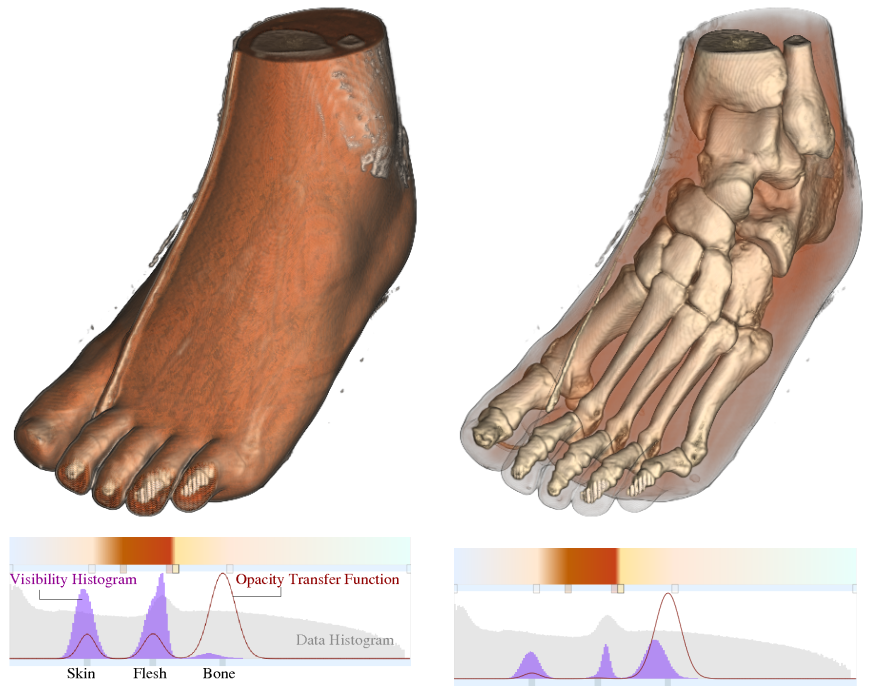
\includegraphics[width=1\linewidth]{images/correa_visibility-driven_2009}
\caption{Visibility histograms for two data sets \cite{correa_visibility-driven_2009}}
\label{fig:correa_visibility-driven_2009}
\end{figure}

With conventional transfer function design, the visibility of certain anatomical structures is a consequence of adjusting transfer function parameters. 
Correa and Ma suggest to control visibility directly by computing visibility histograms as a basis for visibility-driven transfer functions. Visibility-based transfer functions are actually an instance of a data-driven transfer function specification.

%\cite{bordoloi_view_2005}
%\cite{takahashi_feature-driven_2005}


\cite{correa_visibility_2011}
\cite{wang_efficient_2011}

\cite{wan_fast_2010}

\begin{figure}
	\centering
	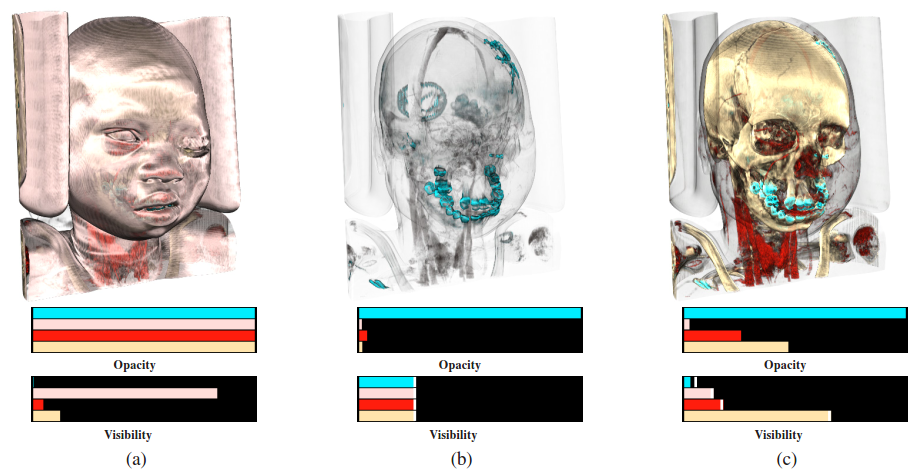
\includegraphics[width=1\linewidth]{images/wang_efficient_2011}
	\caption{Visibility based opacity specification \cite{wang_efficient_2011}}
	\label{fig:wang_efficient_2011}
\end{figure}

\cite{mak_visibility-aware_2011}

\cite{bronstad_visibility_2012}



\cite{ruiz_automatic_2011}
\cite{bramon_information_2013}

\cite{tang_depth-based_2011}
\cite{zhou_opacity_2014}

\section{Multivariate Volume Visualization}
Analyzing multivariate data is an importance and challenging topic in many scientific disciplines. For instance, applications in medicine, engineering and meteorology often require analyzing multivariate data.
However, multivariate volume data sets are usually mapped to a scalar dimension and visualized separately with standard volume rendering techniques.

Kniss and Hansen \cite{kniss_volume_2002} applied volume rendering with multidimensional transfer function to visualize multivariate weather simulations. In their approach, they combined the temperature and humidity as a multivariate field in order to assist the meteorologists in identifying the frontal zones. 

Akiba et al. presented the use of time histogram for simultaneous classification of time-varying data in order to find transfer functions that classify all the time steps of the data set \cite{akiba_simultaneous_2006}.

Woodring and Shen presented a method for the comparison of different data fields through the expression of a volume shader that composes data fields together with set operations \cite{woodring_multi-variate_2006}.

Wang et al. introduced an importance measure based on conditional entropy and categorize temporal behaviors by clustering the importance curves over time \cite{wang_importance-driven_2008}.

Lee and Shen \cite{lee_visualization_2009} extended the Dynamic Time Warping (DTW) approach \cite{lee_visualizing_2009} to SUBDTW, in order to estimate when a trend appears and vanishes in a given time series. They modeled the temporal relationships as a state machine based on the beginning and ending times of the trends.

Khlebnikov et al. \cite{khlebnikov_noise-based_2013} described a novel method that allows simultaneous rendering of multivariate data by redistributing the opacity within a voxel. This method uses procedural texture synthesis \cite{khlebnikov_procedural_2012} for opacity redistribution pattern and is similar in spirit to color weaving.

Data analysis techniques for high dimensional spaces, such as parallel coordinates \cite{akiba_visualizing_2007} \cite{guo_scalable_2012} and principal component analysis \cite{liu_multivariate_2014}, were also investigated for exploring multivariate time-varying data sets.

%\cite{woodring_multi-variate_2006}
%\cite{akiba_visualizing_2007}
%\cite{guo_scalable_2012}
%\cite{liu_multivariate_2014}

\section{Information Theory in Visualization}
Information theory \cite{shannon_mathematical_1948} was originally introduced to study the fundamental limit of reliable transmission of messages through a noisy communication channel. Traditional applications of information theory, such as data compression and data communication, focus on the efficient throughput of a communication channel, whilst visualization focuses on the effectiveness in aiding the perceptual and cognitive process for data understanding and knowledge discovery.

In recent years, there is an emerging direction towards using the principles of information theory to solve challenging problems in scientific visualization \cite{wang_information_2011}. These problems include view selection \cite{bordoloi_view_2005} \cite{takahashi_feature-driven_2005} \cite{feixas_unified_2009}, streamline seeding and selection \cite{xu_information-theoretic_2010} \cite{lee_view_2011}, transfer function for multimodal data \cite{bramon_multimodal_2012}, representative isosurface selection \cite{wang_lod_2006}, time-varying and multivariate data analysis \cite{wang_importance-driven_2008} and information channel between objects and viewpoints \cite{ruiz_viewpoint_2010}.

Chen and J{\"a}nicke \cite{chen_information-theoretic_2010} presented an information-theoretic framework for visualization. They examined the theoretical aspect of information and its relation to data communication and interpret different stages of the visualization pipeline using the taxonomy of information.

Haidacher et at. \cite{haidacher_information-based_2008} proposed an approach of transfer function specification for multi-modal data visualization. They considered the joint occurrence of multiple features from one or multiple variables in order to separate statistical features that only occur in a single variable from those that are present in both.

Want et al. \cite{wang_importance-driven_2008} introduced an approach to characterized the dynamic temporal behaviors of spatial blocks using importance curves, which are based on conditional entropy. Clustering is performed on the importance curves of all the spatial blocks to classify the underlying volume data set.

Ruiz et al. \cite{ruiz_automatic_2011} presented an approach to generate transfer functions from a target distribution provided by the user. Their approach is based on a communication channel between a set of viewpoints and a set of bins of a volume data set, and supports both 1D and 2D transfer functions including the gradient information.

Bramon et al. \cite{bramon_information_2013} proposed an automatic method to visualize multi-modal data by combining several information-theoretic strategies to define colors and opacity values of the multi-modal transfer function.
They set an information channel between two registered input data sets to define the fused color and minimize the informational divergence between the visibility distribution captured by a set of viewpoints and a target distribution proposed by the user to obtain the opacity.

\section{Computational Saliency}
Predicting salient locations has many real world applications, such as navigational assistance, robot control, surveillance systems, object detection and scene understanding \cite{zhao_learning_2013}.
Inspired by mechanisms of the human visual system, various computational models of visual saliency have been proposed to predict gaze allocation \cite{itti_model_1998} \cite{parkhurst_modeling_2002} \cite{harel_graph-based_2006} \cite{chikkerur_what_2010} \cite{mahadevan_spatiotemporal_2010} \cite{duan_visual_2011}.

Lee et al. \cite{lee_mesh_2005} presented mesh saliency, which is defined in a scale-dependent manner using a center-surround operator on Gaussian-weighted mean curvatures. They observed that their approach was able to capture the most visually interesting regions on a mesh.
Kim and Varshney \cite{kim_saliency-guided_2006} introduced the user of center-surround operators to compute saliency fields of volume data. In their user study, they found that their approach was better at eliciting viewer attention than the traditional Gaussian regional enhancement approaches.
Shen et al. \cite{shen_save:_2014} proposed the use of saliency to assist volume exploration. They described a method for inferring interaction position in volume visualization, in order to help users pick focused features conveniently.
Shen et al. \cite{shen_spatiotemporal_2015} described spatiotemporal volume saliency, which extended the saliency field \cite{kim_saliency-guided_2006} to time-varying volume data.

%\cite{kim_mesh_2010}
%\cite{song_mesh_2014}

%A saliency-based enhancement of volume visualization inspired by the center-surround mechanisms of the human
%visual system
%For volume \cite{kim_saliency-guided_2006}
%\cite{kim_saliency-guided_2008}

%saliency assisted
%\cite{wang_saliency-aware_2013}

%\cite{treue_visual_2003}
%\cite{healey_combining_2001}
%\cite{hall_trainable_2004}
%\cite{kadir_saliency_2001}
%\cite{cui_measuring_2006}

\section{Perceptual Evaluation}
Due to the complex nature of the data being studied, simply displaying all available information does not adequately meet the demands of domain scientists \cite{anderson_evaluating_2012}.
%Determining the best use of visualization techniques is one of the goals of visualization evaluations.
User studies can be used to evaluate the strengths and weaknesses of visualization methods \cite{christopher_thoughts_2003}.
The evaluation of visualization methods that focus on human factors often employ user studies or expert evaluations to determine their effects on interpretation and usability.

There are a number of different evaluation strategies, such as measuring user performance, accuracy and experience \cite{redmond_influencing_2010}. Laidlaw et al. \cite{laidlaw_quantitative_2001} compared six methods for visualizing 2D vector fields and measured user performance on three flow-related tasks for each of the six methods. They used the evaluation results to identify what makes a 2D vector fields visualization effective.
Joshi and Rheingans \cite{joshi_evaluation_2008} evaluated the effective of their illustrative techniques by measuring user accuracy, time required to perform a task and user confidence.

Lu \cite{lu_volume_2010} described a method for automatically selecting rendering parameters to simplify user interaction and improve usability. Subsequently, a user study was conducted to evaluate the effectiveness of this method. Two data sets were rendered in three styles with three predefined portions of the data sets were highlighted respectively. The users' eye gaze patterns were analyzed to determine if they were able to accurately identify the highlighted areas in the images.

Kersten-Oertel et al. \cite{kersten-oertel_evaluation_2014} presented empirical studies on the effect of six different perceptual cues for enhancing depth. In the user study, the subjects were asked to determine which one of two indicated vessels was closer to them, and were asked to respond as accurately and quickly as possible. Both the percentage of correct answers and response times were analyzed.

Also for depth perception, D{\'i}az et al. \cite{diaz_perceptual_2015} conducted a user study to investigate the impact of well-known volumetric shading models in stereoscopic desktop-based environments. In the results, the average time spent and average correctness of answers were analyzed.

\section{Feature Tracking}
Feature extraction and tracking is an established technique for the analysis of time-varying data in various research fields, such as video analysis, computer vision and flow visualization \cite{muelder_interactive_2009}.
In time-varying data, features are objects that evolve over time. Feature tracking aims to determine the correspondence between features in successive time steps and describe the evolution of features through time \cite{post_state_2003}.

In practice feature extraction and tracking are often employed in the exploration and analysis of time-varying volume visualization in order to better understand the dynamic nature of the underlying phenomena \cite{tzeng_intelligent_2005} \cite{woodring_multiscale_2009} \cite{lee_visualizing_2009} \cite{gu_transgraph_2011}.
Feature extraction methods are often based on an analytical description of the feature of interest. Consequently, feature extraction and tracking could become a manual-driven and trial-and-error process in the case that the properties cannot be easily defined and are sometimes unknown \cite{ma_machine_2007}.

%%survey
\cite{ma_machine_2007} \cite{wang_information_2008}
%
\cite{caban_texture-based_2007}
%
%%tracking related works
\cite{widanagamaachchi_interactive_2012} \cite{ozer_group_2012}
\cite{hsieh_feature_2013}

\section{Vector Field Visualization}
The visualization of vector fields plays a crucial role in visual interpretation and understand of the underlying flow features and patterns \cite{kuhn_clustering-based_2011} \cite{ma_coherent_2013}. Since flow patterns also exist in time-varying volume data, certain techniques for visualizing vector field could be incorporated into time-varying volume visualization, in order to depict the dynamic aspects of time-varying data.

Line drawings are effective ways to depict complex information with simple means \cite{benard_state_art_2011}. Among vector field visualization techniques, streamline visualization is a simple but common way to convey the structure of 3D vector fields \cite{chen_illustrative_2011}. Streamlines have proven to give expressive visual representation if they are combined with appropriate seeding strategies \cite{annen_vector_2008}. Streamlines intuitively reveal flow patterns by integrating the flow path.

\section{Summary}
We have presented a review of the literature in the field of volume visualization.
The review suggests that it is feasible to optimize the parameters of volume visualization based on the information within the volume data. Existing research on multidimensional transfer functions, classification of volume data and information theory provides us the foundation to explore and understand how this optimization may be achieved.
%Existing research on the analysis and visualization of time-varying data and flow data gives us valuable information on the study of the dynamic aspect of time-varying volume data.
In particular, the analysis and visualization of time-varying data is a compelling problem due to increasing availability of such data in recent years. Although some work has been published in this area, it is clear that there is compelling work left to be done in optimizing the rendering of such data sets.
The use of NPR techniques can improve the expressiveness of the visualization and thus facilitate better user understanding of data.
Further studies are required in order to better integrate NPR techniques into the visualization pipeline and enhance the expressiveness of the visualization by exploiting the information within the data sets.

%-------------------------------------------------------------------------
